\documentclass[tikz,border=5pt]{standalone}
\usepackage{amsmath,amssymb,centernot}
\begin{document}
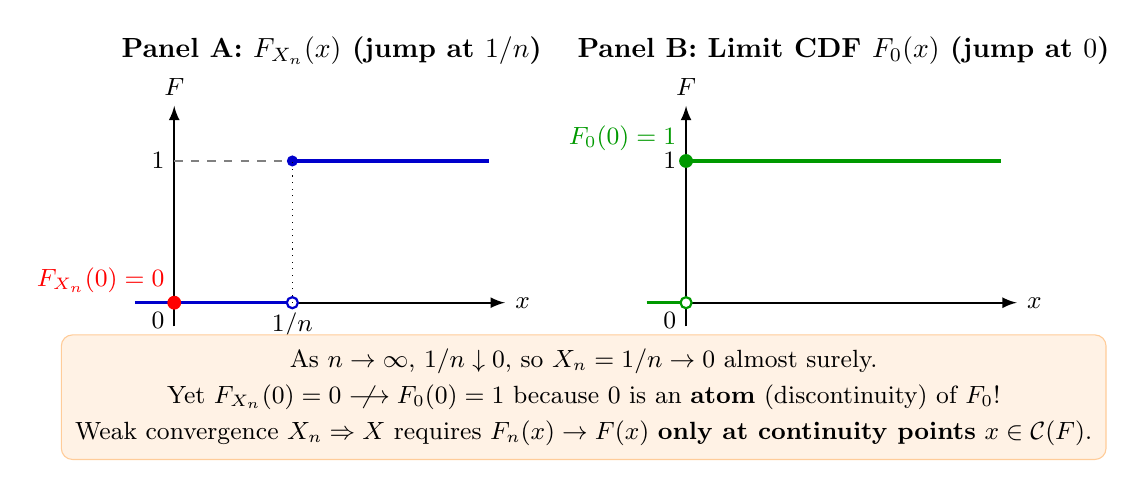
\begin{tikzpicture}[>=latex, font=\small]
  % Panel A: F_{X_n} with jump at 1/n
  \begin{scope}
    \node[font=\bfseries] at (2.0, 3.2) {Panel A: $F_{X_n}(x)$ (jump at $1/n$)};
    \draw[->, thick] (-0.5, 0) -- (4.2, 0) node[right] {$x$};
    \draw[->, thick] (0, -0.3) -- (0, 2.5) node[above] {$F$};

    \node[below left] at (0, 0) {$0$};
    \node[left] at (0, 1.8) {$1$};
    \draw[dashed, gray] (0, 1.8) -- (4, 1.8);

    % Graph of F_{X_n}
    \draw[very thick, blue!80!black] (-0.5, 0) -- (1.5, 0);
    \draw[thick, blue!80!black, fill=white] (1.5, 0) circle (2pt);
    \fill[blue!80!black] (1.5, 1.8) circle (2pt);
    \draw[very thick, blue!80!black] (1.5, 1.8) -- (4.0, 1.8);
    \draw[dotted] (1.5, 0) -- (1.5, 1.8);
    \node[below] at (1.5, 0) {$1/n$};
    \fill[red] (0, 0) circle (2.5pt) node[above left, red] {$F_{X_n}(0) = 0$};
  \end{scope}

  % Panel B: Limit F_0 with jump at 0
  \begin{scope}[xshift=6.5cm]
    \node[font=\bfseries] at (2.0, 3.2) {Panel B: Limit CDF $F_0(x)$ (jump at $0$)};
    \draw[->, thick] (-0.5, 0) -- (4.2, 0) node[right] {$x$};
    \draw[->, thick] (0, -0.3) -- (0, 2.5) node[above] {$F$};

    \node[below left] at (0, 0) {$0$};
    \node[left] at (0, 1.8) {$1$};
    \draw[dashed, gray] (0, 1.8) -- (4, 1.8);

    % Graph of F_0
    \draw[very thick, green!60!black] (-0.5, 0) -- (0, 0);
    \draw[thick, green!60!black, fill=white] (0, 0) circle (2pt);
    \fill[green!60!black] (0, 1.8) circle (2.5pt) node[above left, green!60!black] {$F_0(0) = 1$};
    \draw[very thick, green!60!black] (0, 1.8) -- (4.0, 1.8);
  \end{scope}

  \node[align=center, fill=orange!10, draw=orange!40, rounded corners, inner sep=5pt] at (5.2, -1.2)
    {As $n \to \infty$, $1/n \downarrow 0$, so $X_n = 1/n \to 0$ almost surely.\\[2pt]
     Yet $F_{X_n}(0) = 0 \centernot\longrightarrow F_0(0) = 1$ because $0$ is an \textbf{atom} (discontinuity) of $F_0$!\\[2pt]
     Weak convergence $X_n \Rightarrow X$ requires $F_n(x) \to F(x)$ \textbf{only at continuity points} $x \in \mathcal{C}(F)$.};
\end{tikzpicture}
\end{document}
